\documentclass{beamer}

\usepackage[utf8]{inputenc}
\usepackage[spanish]{babel}
\usepackage[outputdir=.build]{minted}
\usepackage{hyperref}
\usepackage{graphicx}

\hypersetup{
    colorlinks = true
}

\usetheme{Madrid}

%Information to be included in the title page:
\title{Taller de Física Computacional}
\subtitle{Markdown y comentarios}
\author{Cristián G. Sánchez y Carlos J. Ruestes}
\date{2021}

\begin{document}

\frame{\titlepage}

%%%%%%%%%%%%%%%%%%%%%%%%%%%%%%%%%%%%%%%%%%%%%%%%%%%%%%%%%%
\begin{frame}[fragile]
\frametitle{Comentarios}
\begin{block}{Comentarios}
Los comentarios en Python son cualquier cosa que esté después de un carácter numeral, como en el siguiente ejemplo:
\begin{minted}{python}
# Un comentario
# de más de una línea
# se hace con un # en cada una
1 + 1 # todo lo que sigue a # es comentario
'cadena' # esto es una cadena
2**2 + 1 - 1/3 + 0j # qué tipo tendrá esto?
\end{minted}
\end{block}
\end{frame}

%%%%%%%%%%%%%%%%%%%%%%%%%%%%%%%%%%%%%%%%%%%%%%%%%%%%%%%%%%
\begin{frame}[fragile]
\frametitle{Comentarios}
\begin{itemize}
\item No es posible se lo suficientemente enfático en relación a la \alert{absoluta} necesidad de comentar adecuadamente 
todo el código que escribimos.
\item Para variar la página de Wikipedia tiene una excelente revisión de las formas y usos de los comentarios en el código
\item La persona a la que le serán más útiles los comentarios en general es a nosotros mismos\ldots
\end{itemize}
\end{frame}

%%%%%%%%%%%%%%%%%%%%%%%%%%%%%%%%%%%%%%%%%%%%%%%%%%%%%%%%%%
\begin{frame}[fragile]
\frametitle{Markdown en Jupyter}
En el caso de la herramienta Jupyter Notebook, un Notebook es un \alert{documento} y eso nos provee de enormes
posibilidades de enriquecer el código con texto.
\begin{block}{Markdown}
\begin{itemize}
\item {\em Markdown} es un tipo de lenguaje de marcado, como \LaTeX o HTML.
\item En Jupyter Notebook una celda puede contener Markdown.
\item La combinación de Markdown y código convierte un Notebook en un {\bf documento}
\item Es particularmente útil para comunicar resultados o compartir pedazos de programas (explicados) con otros.
\end{itemize}
\end{block}
\end{frame}

%%%%%%%%%%%%%%%%%%%%%%%%%%%%%%%%%%%%%%%%%%%%%%%%%%%%%%%%%%
\begin{frame}[fragile]
\frametitle{Markdown en Google Colab}
\begin{block}{Markdown}
\begin{itemize}
\item Para crear una nueva celda de Markdown desde el menú:  {\em Insert} $\rightarrow$ {\em Text cell}
\item O pulsando el botón {\tt + Text}
\end{itemize}
\end{block}
\begin{figure}
    \centering
    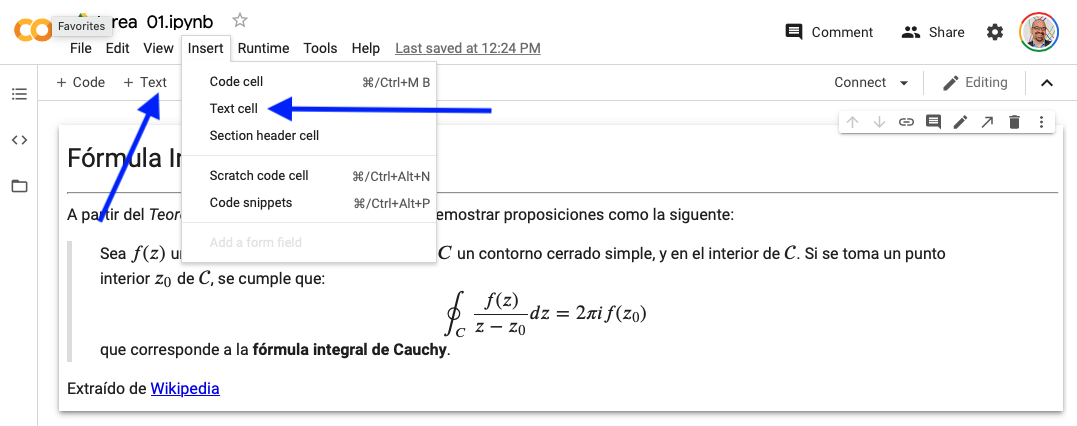
\includegraphics[width=0.9\textwidth]{figuras/colab.png}
\end{figure}


\end{frame}

%%%%%%%%%%%%%%%%%%%%%%%%%%%%%%%%%%%%%%%%%%%%%%%%%%%%%%%%%%%
\begin{frame}
\frametitle{Síntesis y recursos:}

\begin{itemize}
\item Machete que va entre los materiales de esta clase.
\item \href{https://daringfireball.net/projects/markdown/syntax}{La especificación original de John Gruber}
\item \href{https://en.wikipedia.org/wiki/Markdown}{Markdown en Wikipedia}
\item \href{https://jupyter-notebook.readthedocs.io/en/stable/index.html}{Documentación de Jupyter}
\item \href{https://www.python.org/dev/peps/pep-0008/}{Guía de estilo de Python}
\item La funcionalidad de escribir ecuaciones es provista por \href{https://docs.mathjax.org/en/latest/input/tex/}{MathJax} y en la documentación se detallan las diferencias y similitudes con \LaTeX\ y \TeX
\end{itemize}
\end{frame}

\end{document}
